\documentclass[tikz,border=2pt]{standalone}
\usepackage{amsmath}
\usetikzlibrary{arrows.meta}
\begin{document}
% Outside-option game: player 1 takes Out (2,2) or In; then 1 chooses A/B and 2 chooses a/b
% without observing it: (A,a)=(3,1), (B,b)=(1,3), (0,0) otherwise. After In, B gives player 1 at
% most 1 < 2, so player 2 infers A and plays a: forward induction selects (In A, a), payoff (3,1).
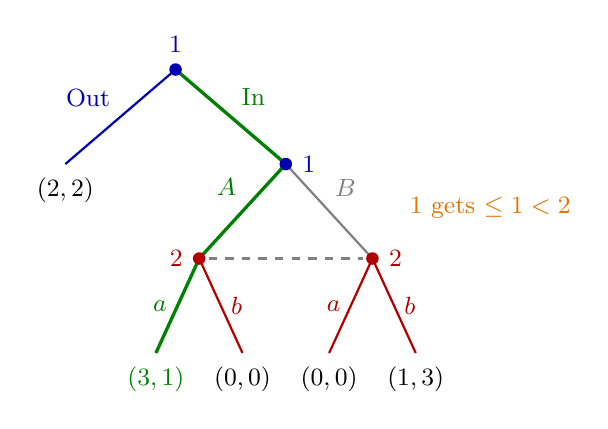
\begin{tikzpicture}[font=\small, >={Latex[length=2mm]},
    dec/.style={circle, fill, inner sep=1.6pt}]
  % edges
  \draw[thick, blue!70!black] (1.9,0) -- node[above left, pos=0.5] {Out} (0.5,-1.2);
  \draw[thick, gray] (3.3,-1.2) -- node[above right, pos=0.45] {$B$} (4.4,-2.4);
  \draw[thick, red!70!black] (2.2,-2.4) -- node[right, pos=0.5] {$b$} (2.75,-3.6);
  \draw[thick, red!70!black] (4.4,-2.4) -- node[left, pos=0.5] {$a$} (3.85,-3.6);
  \draw[thick, red!70!black] (4.4,-2.4) -- node[right, pos=0.5] {$b$} (4.95,-3.6);
  % forward-induction path In, A, a
  \draw[very thick, green!50!black] (1.9,0) -- node[above right, pos=0.5] {In} (3.3,-1.2);
  \draw[very thick, green!50!black] (3.3,-1.2) -- node[above left, pos=0.45] {$A$} (2.2,-2.4);
  \draw[very thick, green!50!black] (2.2,-2.4) -- node[left, pos=0.5] {$a$} (1.65,-3.6);
  % information set of player 2
  \draw[dashed, thick, gray] (2.32,-2.4) -- (4.28,-2.4);
  % nodes
  \node[dec, blue!70!black, label={[blue!70!black]above:$1$}] at (1.9,0) {};
  \node[dec, blue!70!black, label={[blue!70!black]right:$1$}] at (3.3,-1.2) {};
  \node[dec, red!70!black, label={[red!70!black]left:$2$}] at (2.2,-2.4) {};
  \node[dec, red!70!black, label={[red!70!black]right:$2$}] at (4.4,-2.4) {};
  % payoffs
  \node[anchor=north] at (0.5,-1.25) {$(2,2)$};
  \node[anchor=north, green!50!black] at (1.65,-3.65) {$(3,1)$};
  \node[anchor=north] at (2.75,-3.65) {$(0,0)$};
  \node[anchor=north] at (3.85,-3.65) {$(0,0)$};
  \node[anchor=north] at (4.95,-3.65) {$(1,3)$};
  % reasoning
  \node[orange!90!black, anchor=west] at (4.75,-1.75) {1 gets $\le 1<2$};
\end{tikzpicture}
\end{document}
